% !TeX spellcheck = en
\documentclass{article}
\usepackage[utf8]{inputenc}
\usepackage{graphicx}
\usepackage{hyperref}
\usepackage{tikz}
\usepackage{float}
\usepackage[simplified]{pgf-umlcd}
\usetikzlibrary{positioning,fit,calc,arrows.meta, shapes}
\graphicspath{ {images/} }

%Tot això hauria d'anar en un pkg, però no sé com és fa
\newcommand*{\assignatura}[1]{\gdef\1assignatura{#1}}
\newcommand*{\grup}[1]{\gdef\3grup{#1}}
\newcommand*{\professorat}[1]{\gdef\4professorat{#1}}
\renewcommand{\title}[1]{\gdef\5title{#1}}
\renewcommand{\author}[1]{\gdef\6author{#1}}
\renewcommand{\date}[1]{\gdef\7date{#1}}
\renewcommand{\baselinestretch}{1.5}
\renewcommand{\maketitle}{ %fa el maketitle de nou
    \begin{titlepage}
        \raggedright{UNIVERSITAT DE LLEIDA \\
            Escola Politècnica Superior \\
            Grau en Enginyeria Informàtica\\
            \1assignatura\\}
            \vspace{5cm}
            \centering\huge{\5title \\}
            \vspace{3cm}
            \large{\6author} \\
            \normalsize{\3grup}
            \vfill
            Professorat : \4professorat \\
            Data : \7date
\end{titlepage}}
%Emplenar a partir d'aquí per a fer el títol : no se com es fa el package
%S'han de renombrar totes, inclús date, si un camp es deixa en blanc no apareix

\tikzset{
    %Style of nodes. Si poses aquí un estil es pot reutilitzar més facilment
    pag/.style = {circle, draw=black,
                           minimum width=0.75cm, font=\ttfamily,
                           text centered}
}
\title{WebProject: Pre-assignment}
\author{Pau Ibáñez Millán, Joan Martí Olivart, Ian Palacín Aliana, Joaquim Picó Mora, Sergi Simón Balcells}
\date{Diumenge 1 de Març}
\assignatura{Web Project}
\professorat{F. Verdés}
\grup{PraLab1}

%Comença el document
\begin{document}
    \maketitle
    \thispagestyle{empty}
    
    \newpage
    \pagenumbering{roman}
    \tableofcontents
    \newpage
    \pagenumbering{arabic}
    
\section{Our Idea}
In order to find an idea for our web project, we have been looking for a real-world problem to solve. Since in our project team we are all music lovers, we have decided to develop something involved with this topic. \\
Having said that, finally we came up with the following idea: \\
Famous music groups have many facilities and opportunities to show their music anywhere and they have also a big audience that support them, so we wanted to help small music groups to be a little more known or at least allow them to play their music live. \\
Wondering how to achieve this goal, we thought that establishments, such as restaurants or pubs, could be interested in having live music played in their installations for any purpose: inaugurations, parties, special occasions, background music, small concerts, among others. \\
In this way, we will develop a web platform where establishments will post an event announcement and music groups will be able to request to play their music there live. Then, the establishments will decide if they accept these requests, by consulting the music groups profiles in the platform, where they will find what kind of music they play, how many musicians they are, and additional information. \\
Besides this, normal users will be able to see in the platform what events are taking place near them, establishments and music groups profiles, as well as they will be capable of rating (commenting or liking) those profiles and events. \\

\section{API's}
For the same reason mentioned above we have decided to use the SoundCloud API, since it is easier for smaller groups to upload their projects. We had also thought about the Spotify API, but as it requires a pricing for publishing songs in it, and our target are
small music groups, we thought that the freeness of SoundCloud would be better.
\\\\
With this API, when groups create their profile they can share their songs as a portfolio. In this way, when they sign up for a musical event, the organizer can listen to them in order to choose a group.
\newpage
\section{Model}
 \begin{figure}[h]
    \centering
    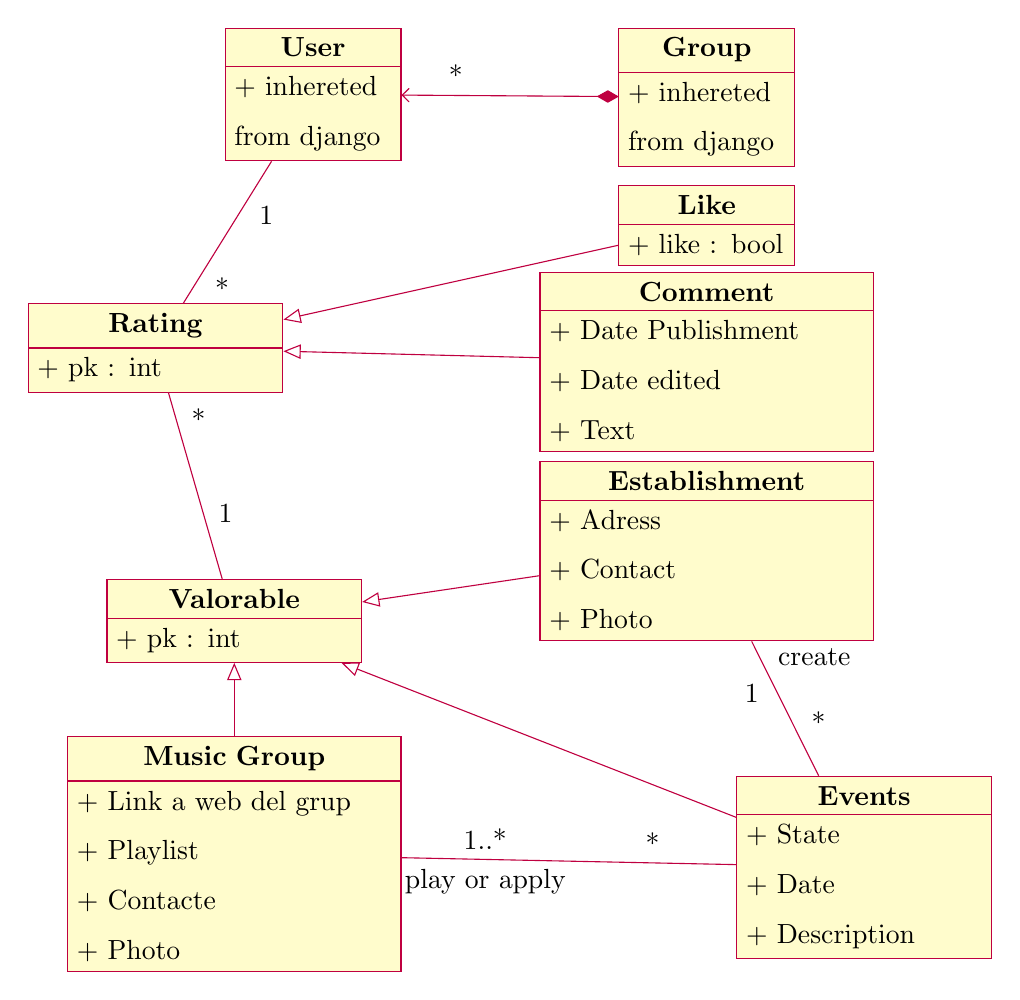
\begin{tikzpicture}
    \begin{class} [text width=3cm]{Valorable}{-1, -7}
    \attribute{+ pk : int}  

    
    \end{class}
    \begin{class} [text width=4cm]{Music Group}{-1, -9}
    \inherit{Valorable} 
        \attribute{+ Link a web del grup}
    \attribute{+ Playlist}
    \attribute{+ Contacte}
    \attribute{+ Photo}

    
    \end{class}
    \begin{class} [text width=4cm]{Establishment}{5, -5.5}
    \inherit{Valorable} 
    
    
    \attribute{+ Adress}
    \attribute{+ Contact}
    \attribute{+ Photo}
    
    \end{class}
    \begin{class} [text width=3cm]{Events}{7, -9.5}
    \inherit{Valorable} 
    
    \attribute{+ State }
    \attribute{+ Date}
    \attribute{+ Description}
    
    \end{class}
    
    \begin{class} [text width=3cm]{Rating}{-2, -3.5}
    \attribute{+ pk : int}  
    
    
    \end{class}
    \begin{class} [text width=4cm]{Comment}{5, -3.1}
    \inherit{Rating}    
    \attribute{+ Date Publishment }
    \attribute{+ Date edited}
    \attribute{+ Text}
    
    
    \end{class}
    \begin{class} [text width=2cm]{Like}{5, -2}
    \inherit{Rating}
    
    
    \attribute{+ like : bool}
    
    \end{class}
    \begin{class} [text width=2cm]{User}{0,0}
    
    \attribute{+ inhereted from django}
    
    \end{class}
    \begin{class} [text width=2cm]{Group}{5, 0}
    
    
    \attribute{+ inhereted from django}
    
    \end{class}
    
    % Assotiations
    \association{User}{1}{}{Rating}{*}{}
    \composition{Group}{}{*}{User}
    \association{Rating}{*}{}{Valorable}{1}{}
    \association{Events}{}{*}{Music Group}{play or apply}{1..*}
    \association{Events}{}{*}{Establishment}{1}{create}
    \end{tikzpicture}
    \caption{Model}
    \end{figure}
\end{document}
    
